\chapter{Full periodogram results} % Main appendix title
\protect\label{chapter:pgramdetail}
\lhead{Appendix \ref{chapter:pgramdetail}. \emph{Periodogram details}}

In this appendix the complete results for the periodicity studies with various treatments of the data and Python
routines are presented.

\section{Equivalent Widths}
\protect\label{section:appewtab}

The following tables, Table \ref{table:origewtaball} and \ref{table:fullewtaball}, present all the periodogram
calculations with the three Python routines employed, with the Original Set of {\harps} data to January 2014 and the
Full Set to March 2016 respectively. The Equivalent Widths are calculated with the Original Set to highlight that the 116-day
period found in \citet{suarezmascareno15} is also returned with those, but not with the Full Set to January 2014.

\begin{table}[!htbp]
\centering
\scalebox{0.75}{
\begin{tabular}{|l|l|r|r|r|r|r|}
\hline
\textbf{Treatment}&\textbf{Routine}&\textbf{Peak 1}&\textbf{Peak 2}&\textbf{Peak 3}&\textbf{Peak 4}&\textbf{Peak 5}\\\hline
None & \scipy & 116.2 & 41.4 & 52.1 & 46.2 & 48.9 \\
 & \astroml & 44.9 & 57.6 & 59.4 & 104.2 & 84.4 \\
 & \gatspy & 49.1 & 41.4 & 49.9 & 57.0 & 116.3 \\\hline
Clipped & \scipy & 118.4 & 57.7 & 106.8 & 105.3 & 44.9 \\
 & \astroml & 45.0 & 51.2 & 57.7 & 47.4 & 84.5 \\
 & \gatspy & 44.9 & 118.4 & 57.8 & 107.2 & 46.4 \\\hline
Binned & \scipy & 41.4 & 53.2 & 110.5 & 62.6 & 116.1 \\
& \astroml & 115.5 & 87.7 & 71.1 & 59.4 & 40.0 \\
& \gatspy & 41.4 & 53.2 & 110.5 & 62.6 & 49.9 \\\hline
Clipped & \scipy & 45.0 & 59.5 & 71.4 & 89.0 & 109.7 \\
binned & \astroml & 59.5 & 45.0 & 71.3 & 49.9 & 51.2 \\
& \gatspy & 45.0 & 59.5 & 71.4 & 89.0 & 107.7 \\\hline
Residuals & \scipy & 116.2 & 41.4 & 48.9 & 52.1 & 53.0 \\
 & \astroml & 45.0 & 59.4 & 57.6 & 84.3 & 104.2 \\
 & \gatspy & 49.1 & 41.4 & 49.9 & 57.0 & 116.3 \\\hline
\end{tabular}}
\caption{This table shows the 5 highest peaks from the periodograms for Equivalent Widths with various treatments of the
  Original Set of data to January 2014.}
\protect\label{table:origewtaball}
\end{table}

\begin{table}[!htbp]
\centering
\scalebox{0.75}{
\begin{tabular}{|l|l|r|r|r|r|r|}
\hline
\textbf{Treatment}&\textbf{Routine}&\textbf{Peak 1}&\textbf{Peak 2}&\textbf{Peak 3}&\textbf{Peak 4}&\textbf{Peak 5}\\\hline
None & \scipy & 49.0 & 41.4 & 62.6 & 56.8 & 53.2 \\
 & \astroml & 114.6 & 123.2 & 108.0 & 83.1 & 91.8 \\
 & \gatspy & 59.2 & 49.0 & 62.6 & 56.9 & 41.4 \\\hline
Clipped & \scipy & 122.2 & 108.0 & 83.1 & 90.2 & 99.1 \\
 & \astroml & 123.1 & 114.9 & 107.8 & 83.1 & 91.8 \\
 & \gatspy & 122.5 & 108.0 & 59.1 & 48.1 & 50.1 \\\hline
Binned & \scipy & 41.4 & 49.0 & 62.6 & 53.3 & 59.2 \\
& \astroml & 123.0 & 114.5 & 91.7 & 101.1 & 107.8 \\
& \gatspy & 41.4 & 59.2 & 49.0 & 62.6 & 53.3 \\\hline
Clipped & \scipy & 114.9 & 123.3 & 108.0 & 87.0 & 83.2 \\
binned & \astroml & 114.8 & 123.2 & 91.7 & 107.7 & 87.0 \\
& \gatspy & 114.9 & 123.3 & 108.0 & 87.0 & 83.2 \\\hline
Residuals & \scipy & 49.0 & 41.4 & 62.6 & 56.8 & 53.3 \\
 & \astroml & 114.6 & 123.2 & 108.0 & 83.1 & 91.8 \\
 & \gatspy & 59.2 & 49.0 & 62.6 & 56.9 & 41.4 \\\hline
\end{tabular}}
\caption{This table shows the 5 highest peaks from the periodograms for Equivalent Widths with various treatments of the
  Full Set of data to March 2916.}
\protect\label{table:fullewtaball}
\end{table}

In these tables where spectra are clipped as having Equivalent Width over one standard deviation above the median, this
is to the values given in Table \ref{table:ewtabfirst}, i.e. 3.8 for the Original Set to 2014 and 4.2 for the Full Set
to 2016.

The residual Equivalent Widths are calculated by dividing by the mean of the 5 spectra with the smallest {\ha}
Equivalent Widths. These spectra were ones timed at 5 April 2011 UTC 03:26:33 (the lowest), 16 March 2006 UTC 06:37:59,
14 March 2007 UTC 07:28:29, 8 April 2011 UTC 06:28:17 and 22 April 2011 UTC 05:07:46.

\section{{\ha} Index measurement}
\protect\label{section:apphaitab}

In Table \ref{table:bothhaitable} is shown the results for all three Python routines used evaluating the {\ha} Index.
These are calculated with the Original Set of data to 2014 as well as the Full Set to 2016 to highlight that the 116-day
period found in \citet{suarezmascareno15} with the Original Set, but not with the Full Set to January 2014.

\begin{table}[!htbp]
\centering
\scalebox{0.75}{
\begin{tabular}{|l|l|r|r|r|r|r|}
\hline
\textbf{Data}&\textbf{Routine}&\textbf{Peak 1}&\textbf{Peak 2}&\textbf{Peak 3}&\textbf{Peak 4}&\textbf{Peak 5}\\\hline
Set to 2014 & \scipy & 116.2 & 41.4 & 52.1 & 48.9 & 53.0 \\
 & \astroml & 45.0 & 51.2 & 57.6 & 84.5 & 116.6 \\
 & \gatspy & 49.1 & 41.4 & 49.9 & 57.0 & 116.3 \\\hline
Full Set & \scipy & 49.0 & 41.4 & 62.6 & 56.8 & 53.3 \\
 & \astroml & 123.2 & 114.7 & 107.9 & 83.1 & 87.0 \\
 & \gatspy & 59.2 & 49.0 & 62.6 & 56.9 & 41.4 \\\hline
\end{tabular}}
\caption{This table shows the 5 highest peaks from the periodograms for the Original and Full Sets of Data.}
\protect\label{table:bothhaitable}
\end{table}

\section{{\ha} Peak Ratio measurments}
\protect\label{section:appprtab}

The following tables, Table \ref{table:origprtaball} and \ref{table:fullprtaball}, present all the periodogram
calculations with the three Python routines employed, with the Original Set of {\harps} data to January 2014 and the
Full Set to March 2016 respectively. The Peak Ratios are calculated with the Original Set to highlight that the 116-day
period found in \citet{suarezmascareno15} for the {\ha} Index measurement (and also with the Equivalent Widths, see
Section \ref{section:appewtab} is not returned with this measurement.

\begin{table}[!htbp]
\centering
\scalebox{0.75}{
\begin{tabular}{|l|l|r|r|r|r|r|}
\hline
\textbf{Treatment}&\textbf{Routine}&\textbf{Peak 1}&\textbf{Peak 2}&\textbf{Peak 3}&\textbf{Peak 4}&\textbf{Peak 5}\\\hline
None & \scipy & 41.9 & 92.4 & 81.1 & 49.7 & 44.1 \\
 & \astroml & 80.0 & 103.9 & 92.5 & 49.2 & 45.5 \\
 & \gatspy & 81.0 & 41.9 & 92.4 & 103.9 & 44.1 \\\hline
Clipped & \scipy & 41.9 & 81.3 & 49.8 & 92.1 & 44.1 \\
 & \astroml & 49.9 & 41.9 & 91.9 & 101.5 & 58.1 \\
 & \gatspy & 81.2 & 41.9 & 49.8 & 92.2 & 44.1 \\\hline
Binned & \scipy & 82.2 & 61.0 & 80.9 & 49.6 & 40.6 \\
 & \astroml & 71.1 & 115.2 & 80.0 & 91.8 & 123.2 \\
 & \gatspy & 82.3 & 61.0 & 49.4 & 81.0 & 40.6 \\\hline
Clipped & \scipy & 82.2 & 61.1 & 40.5 & 81.0 & 115.8 \\
binned & \astroml & 108.0 & 71.2 & 80.0 & 57.1 & 65.5 \\
 & \gatspy & 82.2 & 61.1 & 40.5 & 81.0 & 49.3 \\\hline
Residuals & \scipy & 41.9 & 41.4 & 49.7 & 92.4 & 44.2 \\
 & \astroml & 45.4 & 80.0 & 84.1 & 92.6 & 49.2 \\
 & \gatspy & 41.9 & 45.5 & 49.8 & 41.4 & 80.9 \\\hline
\end{tabular}}
\caption{This table shows the 5 highest peaks from the periodograms for Peak Ratios with various treatments of the Original Set of data to January 2014.}
\protect\label{table:origprtaball}
\end{table}

\begin{table}[!htbp]
\centering
\scalebox{0.75}{
\begin{tabular}{|l|l|r|r|r|r|r|}
\hline
\textbf{Treatment}&\textbf{Routine}&\textbf{Peak 1}&\textbf{Peak 2}&\textbf{Peak 3}&\textbf{Peak 4}&\textbf{Peak 5}\\\hline
None & \scipy & 121.7 & 123.3 & 83.0 & 114.6 & 90.1 \\
 & \astroml & 60.6 & 52.1 & 49.1 & 56.9 & 57.9 \\
 & \gatspy & 121.8 & 49.9 & 114.7 & 83.0 & 42.0 \\\hline
Clipped & \scipy & 122.3 & 91.8 & 83.0 & 115.0 & 42.0 \\
 & \astroml & 60.8 & 73.0 & 102.0 & 79.5 & 56.8 \\
 & \gatspy & 122.5 & 58.1 & 47.5 & 83.0 & 91.7 \\\hline
Binned & \scipy & 82.2 & 40.6 & 51.1 & 63.6 & 66.8 \\
 & \astroml & 91.6 & 60.9 & 87.0 & 79.3 & 122.0 \\
 & \gatspy & 82.2 & 40.6 & 51.1 & 63.6 & 48.0 \\\hline
Clipped & \scipy & 40.5 & 80.9 & 48.1 & 116.7 & 51.1 \\
binned & \astroml & 114.8 & 91.4 & 122.1 & 122.7 & 107.4 \\
 & \gatspy & 40.5 & 80.9 & 48.1 & 119.9 & 116.7 \\\hline
Residuals & \scipy & 121.6 & 123.7 & 49.8 & 90.0 & 83.0 \\
 & \astroml & 60.6 & 73.1 & 79.6 & 65.0 & 57.0 \\
 & \gatspy & 121.7 & 49.9 & 123.7 & 58.0 & 47.5 \\\hline
\end{tabular}}
\caption{This table shows the 5 highest peaks from the periodograms for Peak Ratios with various treatments of the
  Full Set of data to March 2916.}
\protect\label{table:fullprtaball}
\end{table}

In these tables the clipping, binning and calculation of residuals is exactly as described above for Equivalent Widths
in Section \ref{section:appewtab}.

\section{Skewness and Kurtosis measurements}
\protect\label{section:appkstab}

The following tables, Table \ref{table:origskewtaball} and \ref{table:origkurttaball} present the periodogram
calculations with the three Python routines employed, with the Original Set of {\harps} data to January 2014. Following
these the Tables \ref{table:fullskewtaball} and \ref{table:fullkurttaball} present the periodogram calculations for the
Full Set of data to March 2016.

As with the Equivalent Widths in Section \ref{section:appewtab}, the calculation is performed for the Original Set of data as
the 116-day period found in \citet{suarezmascareno15} again appears, even in this case after clipping, binning or both
is attempted.

\begin{table}[!htbp]
\centering
\scalebox{0.75}{
\begin{tabular}{|l|l|r|r|r|r|r|}
\hline
\textbf{Treatment}&\textbf{Routine}&\textbf{Peak 1}&\textbf{Peak 2}&\textbf{Peak 3}&\textbf{Peak 4}&\textbf{Peak 5}\\\hline
None & \scipy & 122.8 & 98.3 & 87.6 & 117.2 & 106.0 \\
 & \astroml & 87.7 & 116.8 & 105.5 & 122.4 & 79.7 \\
 & \gatspy & 87.7 & 116.8 & 105.5 & 122.4 & 79.7 \\\hline
Clipped & \scipy & 98.2 & 122.9 & 65.3 & 71.3 & 59.7 \\
 & \astroml & 87.5 & 65.5 & 115.8 & 79.8 & 98.2 \\
 & \gatspy & 87.5 & 65.5 & 115.8 & 79.8 & 98.2 \\\hline
Binned & \scipy & 105.7 & 117.7 & 87.8 & 103.3 & 79.6 \\
 & \astroml & 105.7 & 117.7 & 87.8 & 103.3 & 48.8 \\
 & \gatspy & 105.7 & 117.7 & 87.8 & 103.3 & 48.8 \\\hline
Clipped & \scipy & 59.6 & 87.7 & 117.1 & 65.5 & 105.6 \\
binned & \astroml & 59.6 & 87.7 & 117.0 & 65.5 & 105.6 \\
 & \gatspy & 59.6 & 87.7 & 117.0 & 65.5 & 105.6 \\\hline
Residuals & \scipy & 71.8 & 73.8 & 57.7 & 93.0 & 98.4 \\
 & \astroml & 93.1 & 83.7 & 74.1 & 52.2 & 71.9 \\
 & \gatspy & 93.1 & 83.7 & 74.1 & 52.2 & 71.9 \\\hline
\end{tabular}}
\caption{This table shows the 5 highest peaks from the periodograms for Skewness with various treatments of the Original
  Set of data to January 2014.}
\protect\label{table:origskewtaball}
\end{table}

\begin{table}[!htbp]
\centering
\scalebox{0.75}{
\begin{tabular}{|l|l|r|r|r|r|r|}
\hline
\textbf{Treatment}&\textbf{Routine}&\textbf{Peak 1}&\textbf{Peak 2}&\textbf{Peak 3}&\textbf{Peak 4}&\textbf{Peak 5}\\\hline
None & \scipy & 117.2 & 122.7 & 106.4 & 87.2 & 103.6 \\
 & \astroml & 116.7 & 80.9 & 87.3 & 105.2 & 103.7 \\
 & \gatspy & 116.7 & 80.9 & 87.3 & 105.2 & 103.7 \\\hline
Clipped & \scipy & 117.2 & 87.3 & 59.6 & 65.4 & 122.5 \\
 & \astroml & 116.8 & 80.9 & 87.5 & 65.5 & 59.8 \\
 & \gatspy & 116.8 & 80.9 & 87.5 & 65.5 & 59.8 \\\hline
Binned & \scipy & 116.5 & 105.3 & 88.8 & 103.7 & 87.6 \\
 & \astroml & 116.4 & 105.3 & 103.8 & 88.8 & 87.6 \\
 & \gatspy & 116.4 & 105.3 & 103.8 & 88.8 & 87.6 \\\hline
Clipped & \scipy & 59.6 & 117.9 & 45.0 & 80.9 & 87.8 \\
binned & \astroml & 59.6 & 118.1 & 81.0 & 105.7 & 45.0 \\
 & \gatspy & 59.6 & 118.1 & 81.0 & 105.7 & 45.0 \\\hline
Residuals & \scipy & 117.6 & 106.6 & 103.5 & 74.0 & 51.4 \\
 & \astroml & 117.4 & 81.1 & 106.3 & 57.3 & 103.5 \\
 & \gatspy & 117.4 & 81.1 & 106.3 & 57.3 & 103.5 \\\hline
\end{tabular}}
\caption{This table shows the 5 highest peaks from the periodograms for Kurtosis with various treatments of the Original
  Set of data to January 2014.}
\protect\label{table:origkurttaball}
\end{table}

\begin{table}[!htbp]
\centering
\scalebox{0.75}{
\begin{tabular}{|l|l|r|r|r|r|r|}
\hline
\textbf{Treatment}&\textbf{Routine}&\textbf{Peak 1}&\textbf{Peak 2}&\textbf{Peak 3}&\textbf{Peak 4}&\textbf{Peak 5}\\\hline
None & \scipy & 121.9 & 83.4 & 60.0 & 79.1 & 106.4 \\
 & \astroml & 83.4 & 122.2 & 60.0 & 63.4 & 77.7 \\
 & \gatspy & 83.4 & 122.2 & 60.0 & 63.4 & 77.7 \\\hline
Clipped & \scipy & 121.9 & 99.1 & 59.9 & 83.3 & 65.1 \\
 & \astroml & 59.9 & 63.3 & 77.8 & 83.3 & 113.5 \\
 & \gatspy & 59.9 & 63.3 & 77.8 & 83.3 & 113.5 \\\hline
Binned & \scipy & 106.8 & 79.2 & 85.8 & 121.5 & 64.8 \\
 & \astroml & 106.8 & 79.2 & 85.8 & 121.6 & 64.8 \\
 & \gatspy & 106.8 & 79.2 & 85.8 & 121.6 & 64.8 \\\hline
Clipped & \scipy & 59.7 & 71.9 & 85.9 & 41.4 & 77.6 \\
binned & \astroml & 59.7 & 71.9 & 85.9 & 41.4 & 107.0 \\
 & \gatspy & 59.7 & 71.9 & 85.9 & 41.4 & 107.0 \\\hline
Residuals & \scipy & 121.5 & 98.6 & 108.2 & 90.2 & 105.9 \\
 & \astroml & 108.2 & 121.8 & 105.8 & 90.1 & 83.4 \\
 & \gatspy & 108.2 & 121.8 & 105.8 & 90.1 & 83.4 \\\hline
\end{tabular}}
\caption{This table shows the 5 highest peaks from the periodograms for Skewness with various treatments of the Full
  Set of data to March 2016.}
\protect\label{table:fullskewtaball}
\end{table}

\begin{table}[!htbp]
\centering
\scalebox{0.75}{
\begin{tabular}{|l|l|r|r|r|r|r|}
\hline
\textbf{Treatment}&\textbf{Routine}&\textbf{Peak 1}&\textbf{Peak 2}&\textbf{Peak 3}&\textbf{Peak 4}&\textbf{Peak 5}\\\hline
None & \scipy & 122.8 & 86.8 & 83.1 & 114.4 & 79.4 \\
 & \astroml & 122.9 & 114.6 & 86.8 & 86.0 & 83.0 \\
 & \gatspy & 122.9 & 114.6 & 86.8 & 86.0 & 83.0 \\\hline
Clipped & \scipy & 122.9 & 86.9 & 114.5 & 65.1 & 83.1 \\
 & \astroml & 114.7 & 86.9 & 122.9 & 86.1 & 59.9 \\
 & \gatspy & 114.7 & 86.9 & 122.9 & 86.1 & 59.9 \\\hline
Binned & \scipy & 114.6 & 121.9 & 107.5 & 86.8 & 101.3 \\
 & \astroml & 114.6 & 107.5 & 121.9 & 86.8 & 101.4 \\
 & \gatspy & 114.6 & 107.5 & 121.9 & 86.8 & 101.4 \\\hline
Clipped & \scipy & 114.8 & 107.6 & 122.4 & 86.9 & 59.8 \\
binned & \astroml & 114.8 & 107.6 & 122.4 & 86.8 & 59.8 \\
 & \gatspy & 114.8 & 107.6 & 122.4 & 86.8 & 59.8 \\\hline
Residuals & \scipy & 106.9 & 51.4 & 85.4 & 82.6 & 122.2 \\
 & \astroml & 85.5 & 51.4 & 106.9 & 82.5 & 60.0 \\
 & \gatspy & 85.5 & 51.4 & 106.9 & 82.5 & 60.0 \\\hline
\end{tabular}}
\caption{This table shows the 5 highest peaks from the periodograms for Kurtosis with various treatments of the Full
  Set of data to March 2016.}
\protect\label{table:fullkurttaball}
\end{table}

\section{TiO line measurments}
\protect\label{section:apptiotab}

For comparison with the measurements on {\ha}, some similar calculations were done with the TiO peak highlighted in
Fig. \ref{fig:harpsfirstha}, right panel. In Fig. \ref{fig:tiopeak}, this is shown to larger scale.

\begin{figure}[!htbp]
\begin{center}
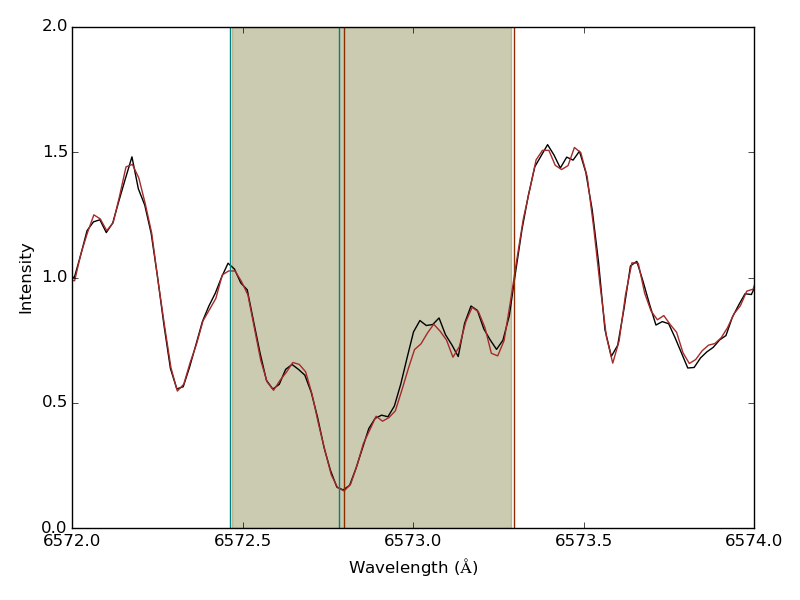
\includegraphics[scale=0.25]{Figures/tipeak.png} \\
\end{center}   
\caption{Enlargement of the TiO absorption peak shown in the right panel of Fig. \ref{fig:harpsfirstha}. The two spectra
highlighted are from the spectra in the left panel of that figure, i.e. 27 May 2004 02:10:14 UTC (black) and 15 March
2006 09:16:35 (brown). Shaded is the area used for calculation of the Equivalent Width and the red and blue lines
delineate the regions used for Peak Ratio calculations.}
 \protect\label{fig:tiopeak}
\end{figure}

\begin{table}[!htbp]
\centering
\scalebox{0.75}{
\begin{tabular}{|l|l|r|r|r|r|r|}
\hline
\textbf{Treatment}&\textbf{Routine}&\textbf{Peak 1}&\textbf{Peak 2}&\textbf{Peak 3}&\textbf{Peak 4}&\textbf{Peak 5}\\\hline
Original data & \scipy & 104.4 & 71.0 & 55.5 & 57.4 & 73.5 \\
EW & \astroml & 71.0 & 68.1 & 89.0 & 104.8 & 43.5 \\
 & \gatspy & 68.1 & 71.0 & 104.5 & 105.4 & 75.0 \\\hline
Original data & \scipy & 70.9 & 49.6 & 67.9 & 89.1 & 104.1 \\
EW & \astroml & 71.0 & 51.2 & 76.3 & 49.8 & 89.1 \\
Binned & \gatspy & 70.9 & 49.6 & 67.9 & 104.2 & 89.1 \\\hline
Original data & \scipy & 94.2 & 88.6 & 105.2 & 99.5 & 42.3 \\
PR & \astroml & 88.1 & 76.0 & 105.2 & 99.9 & 121.4 \\
 & \gatspy & 88.2 & 88.6 & 105.9 & 71.2 & 94.0 \\\hline
Original data & \scipy & 74.0 & 99.3 & 71.9 & 68.9 & 92.6 \\
PR & \astroml & 76.1 & 57.9 & 88.7 & 53.3 & 95.0 \\
binned & \gatspy & 99.1 & 73.8 & 71.8 & 120.1 & 121.8 \\\hline
Full data & \scipy & 97.6 & 106.2 & 109.5 & 44.3 & 70.8 \\
EW & \astroml & 42.4 & 40.8 & 46.1 & 54.1 & 50.9 \\
 & \gatspy & 106.2 & 46.0 & 97.1 & 44.2 & 75.0 \\\hline
Full data & \scipy & 121.6 & 43.6 & 40.7 & 49.5 & 108.9 \\
EW & \astroml & 47.0 & 54.2 & 49.8 & 59.4 & 43.7 \\
Binned & \gatspy & 121.6 & 43.6 & 40.7 & 49.5 & 109.0 \\\hline
Full data & \scipy & 50.6 & 42.2 & 68.0 & 106.3 & 46.1 \\
PR & \astroml & 54.1 & 46.1 & 51.6 & 60.2 & 47.0 \\
 & \gatspy & 46.1 & 68.0 & 63.1 & 50.5 & 42.3 \\\hline
Full data & \scipy & 98.2 & 121.7 & 107.6 & 106.3 & 120.4 \\
PR & \astroml & 65.8 & 47.0 & 54.1 & 71.4 & 76.6 \\
binned & \gatspy & 121.0 & 98.5 & 107.6 & 106.4 & 44.5 \\\hline
\end{tabular}}
\caption{This table shows the 5 highest peaks from the periodograms for various treatments of the TiO peak highlighted
  in Fig. \ref{fig:tiopeak} for Original and Full Sets of {\harps} data.}
\protect\label{table:tipeakall}
\end{table}
